% Present the findings of your research. Provide a detailed 
% analysis of the performance of the various algorithms used 
% for weather prediction, including their accuracy, precision, 
% and recall rates.

% The results section of your thesis presents the findings of 
% your study. It should provide a clear and concise summary of 
% the data collected and analyzed, along with any statistical 
% tests or other methods used to analyze the data. Here are some 
% important elements to consider including in your results section:

% Overall, the results section of your thesis should provide a 
% clear and concise summary of your findings, along with any statistical 
% tests or other methods used to analyze the data. It should also provide 
% an interpretation of your findings and relate them back to your research 
% questions or hypotheses.
\section{Wyniki}

% Descriptive statistics: Provide descriptive statistics that 
% summarize the main characteristics of your data, such as means, 
% standard deviations, and frequency distributions.
\subsection{Statystyki}

Jak widać na rysunku \ref{mse}, w przypadku każdego algorytmu nastąpił
spadek dokładności względem danych testowych. W przypadku modelu KNN oraz
regresji gaussowskiej znikomy błąd na danych treningowych wynika z faktu, 
że obydwa modele bazują na uczeniu na przykładach i ich ewaluacja na 
danych treningowych jest niemiarodajna. 

\begin{figure}[H]
    \centering
    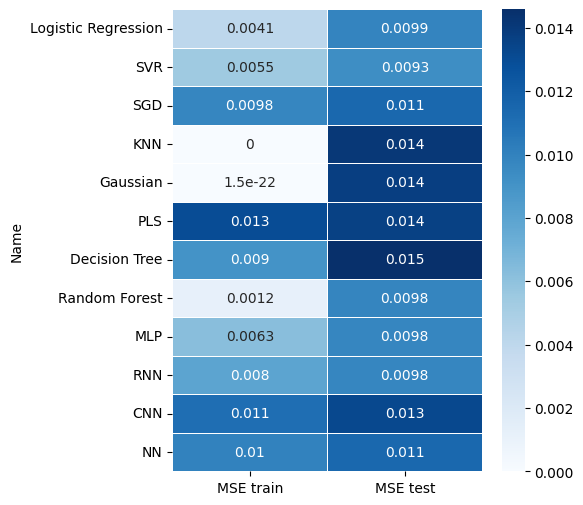
\includegraphics[width=\textwidth]{images/mse.png}
    \caption{Błąd średniokwadratowy dla stworzonych modeli}
    \label{mse}
\end{figure}

Las losowy okazuję się algorytmem, który jest w stanie bardzo dobrze 
dopasować się do danych treningowych razem z zachowaniem ogólności dla 
reszty danych, osiągając dobre wyniki na zbiorze testowym. Z kolei RNN, NN
SVR osiągają zbliżone wartości zarówno dla zbioru treningowego, jak i testowego.

\begin{figure}[H]
    \centering
    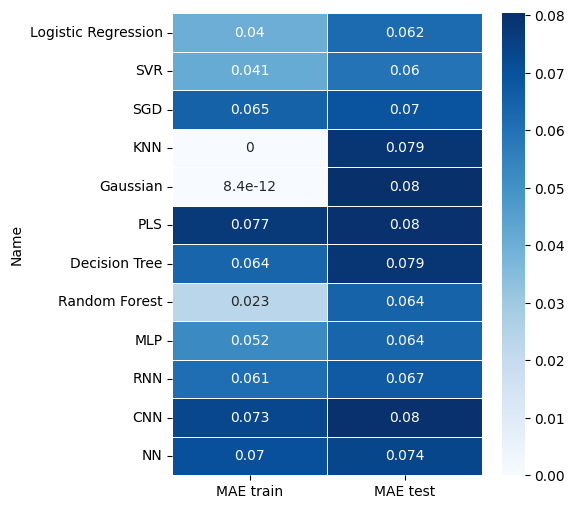
\includegraphics[width=\textwidth]{images/mae.png}
    \caption{Średni błąd absolutny dla stworzonych modeli}
    \label{mae}
\end{figure}

Wartości błędu absolutnego osiągają większe wartości od MSE. Co więcej,
rozbieżność między błędem dla zbioru treningowego i testowego
przy użyciu metryki MAE staje się mniejsza. Ogólna dystrybucja błędu 
względem modeli zdaje się podobna.

\begin{figure}[H]
    \centering
    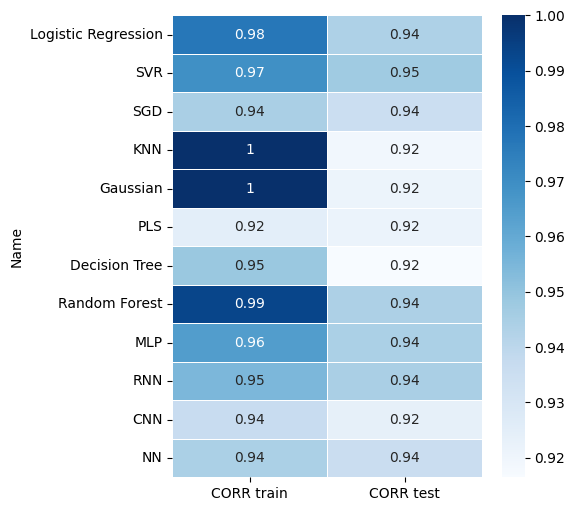
\includegraphics[width=\textwidth]{images/corr.png}
    \caption{Współczynnik korelacji dla stworzonych modeli}
    \label{corr}
\end{figure}

Dla wszystkich modeli współczynnik korelacji pomiędzy wartościami rzeczywistymi 
a przewidzianymi jest na poziomie przekraczającym 0,9. Wskazuje to na dobre dopasowanie
modeli do przewidzianych danych, chociaż warto wskazać, że współczynnik
autokorelacji dla wielu parametrów pozostawał na poziomie powyżej 0,8 dla wartości
opóźnienia przekraczających parę godzin.

\begin{figure}[H]
    \centering
    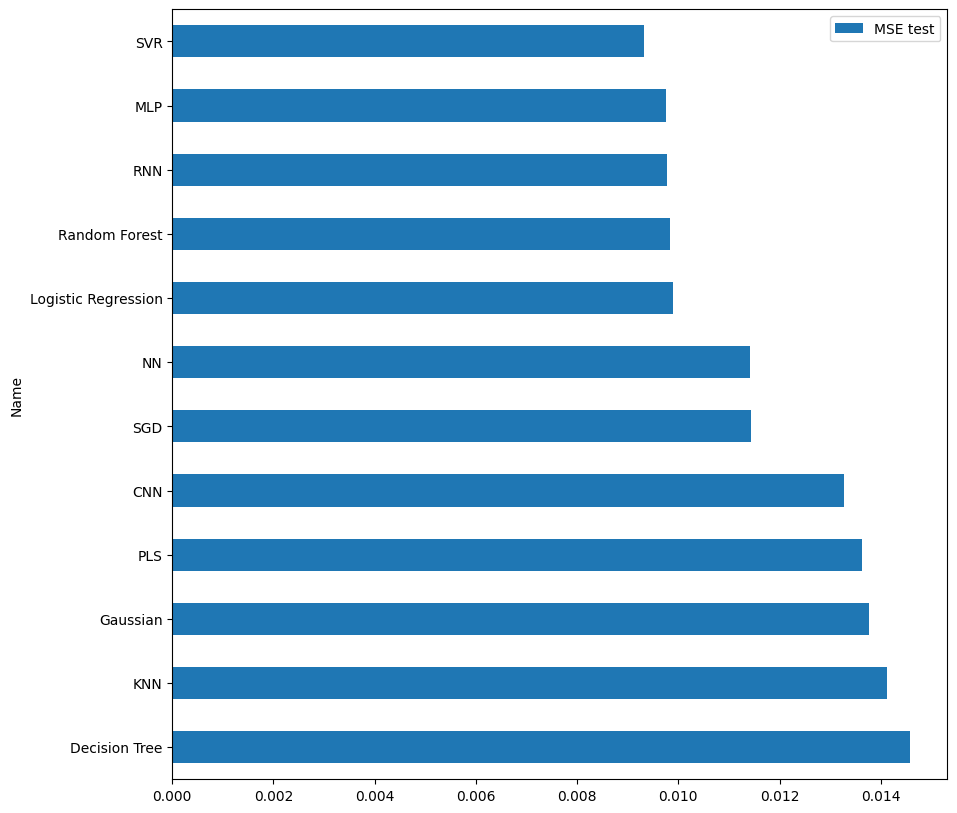
\includegraphics[width=\textwidth]{images/mse_ranking.png}
    \caption{Ranking stworzonych modeli ze względu na błąd średniokwadratowy}
    \label{mse-ranking}
\end{figure}

Na wykresie \ref{mse-ranking} widać stworzony ranking ze względu na wartość MSE.
Najlepszymi algorytmami pod tym względem okazały się SVR, MLP i RNN. Rozbieżność 
pomiędzy najlepszym modelem a najgorszym wynosiła 0,0057. Algorytmami 
osiągającymi najgorsze wyniki był KNN i drzewo decyzyjne.

Można przeprowadzić podobną analizę ze względu na MAE, co zostało pokazane na 
rysunku \ref{mae-ranking}. W tym przypadku o wiele lepsze wyniki 
otrzymała regresja logistyczna i las losowy, które znajdują się wśród najlepiej 
ocenionych algorytmów.

\begin{figure}[H]
    \centering
    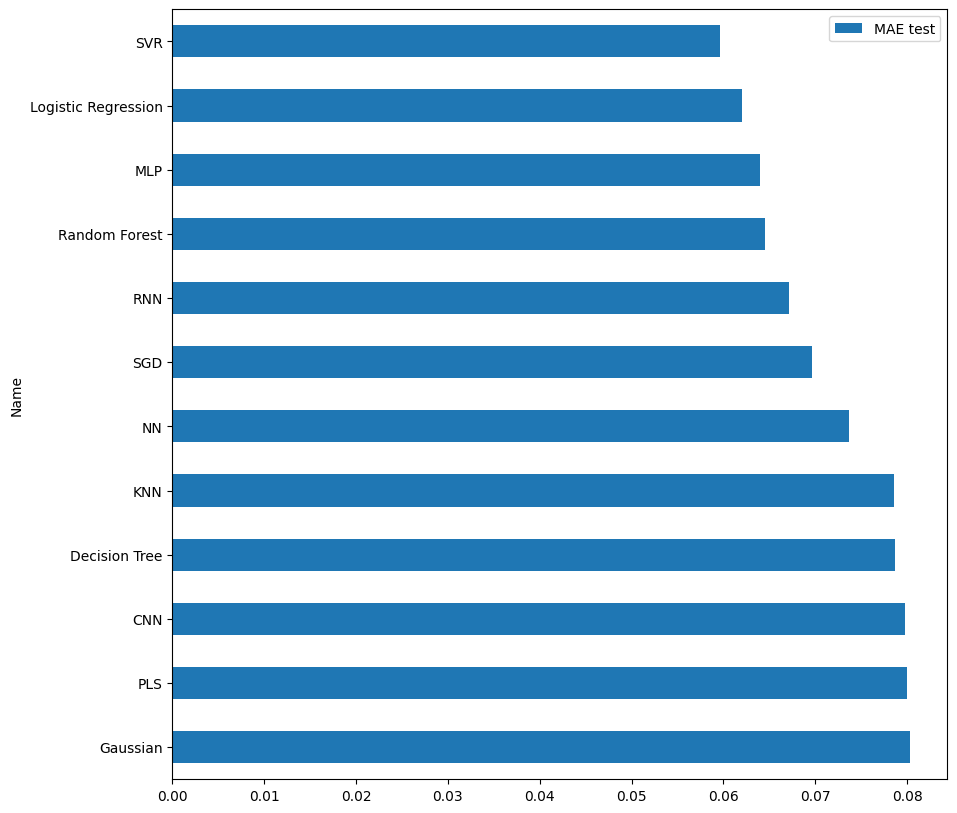
\includegraphics[width=\textwidth]{images/mae_ranking.png}
    \caption{Ranking stworzonych modeli ze względu na średni błąd absolutny}
    \label{mae-ranking}
\end{figure}

Analiza ze względu na korelację pokazuje bardzo zbliżone wartości dla wszystkich 
modeli, a kolejność algorytmów w pokazanym rankingu \ref{corr-ranking} jest 
bardzo podobna do tej ze względu na błąd średniokwadratowy \ref{mse-ranking}.

\begin{figure}[H]
    \centering
    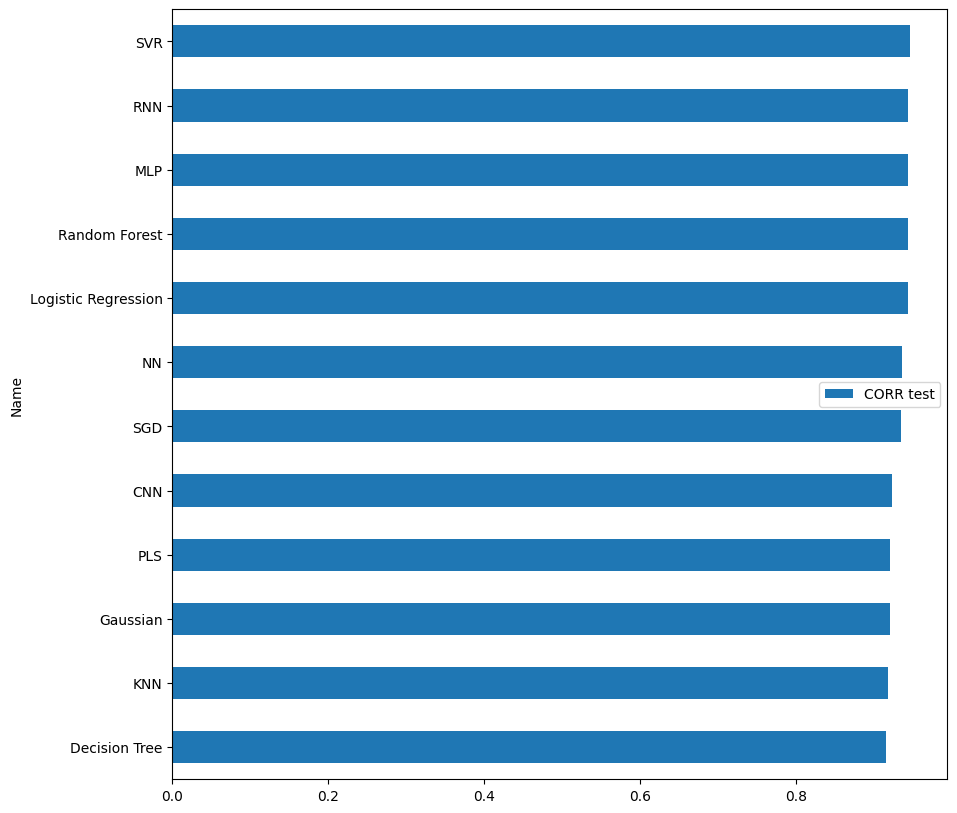
\includegraphics[width=\textwidth]{images/corr_ranking.png}
    \caption{Ranking stworzonych modeli ze względu na wartość korelacji}
    \label{corr-ranking}
\end{figure}

W celu dalszego przybliżenia zachowania poszczególnych modeli, stworzone zostały
zestawienia prawdziwych przebiegów czasowych oraz tych wygenerowanych przez algorytmy
uczenia maszynowego. Chociaż zaprezentowane metryki dają wstępne zrozumienie
stopnia dopasowania modeli oraz ich dokładności, to analiza graficzna jest kluczowa
do zrozumienia, jakie zjawiska są dobrze prognozowane, a jakie stwarzają problemy.
Przedstawione przebiegi prezentują tygodniowe przebiegi złożone z siedmiu 
dwudziestoczterogodzinnych prognoz.

\pagebreak

Jednym z najlepiej ocenianych algorytmów była regresja wektorów wspierających.
W tym przypadku widzimy dobre zachowanie względem przebiegów cyklicznych, takich jak
promieniowanie słoneczne czy odparowanie. Pod względem promieniowania termicznego
widoczne jest dobre odwzorowanie wartości średniej szeregu czasowego, lecz problem
z dopasowaniem do indywidualnych skoków w wartościach.

Nagły skok w wartości opadów został zupełnie pominięty w prognozie i wskazuje 
na problemy z przewidywaniem nagłych zdarzeń o dużej amplitudzie. 

Zarówno wartości prędkości wiatru, jak i temperatury zostały wiernie odwzorowane
przez stworzony model, a na poniższych wykresach widać jak linie prognozowanych wartości
podążają za wartościami przewidywanymi. W przypadku ciśnienia atmosferycznego,
po nagłym spadku model był w stanie dopasować się ponownie do danych pomiarowych
i dalej podążać za utworzonym trendem.

\begin{figure}[H]
    \centering
    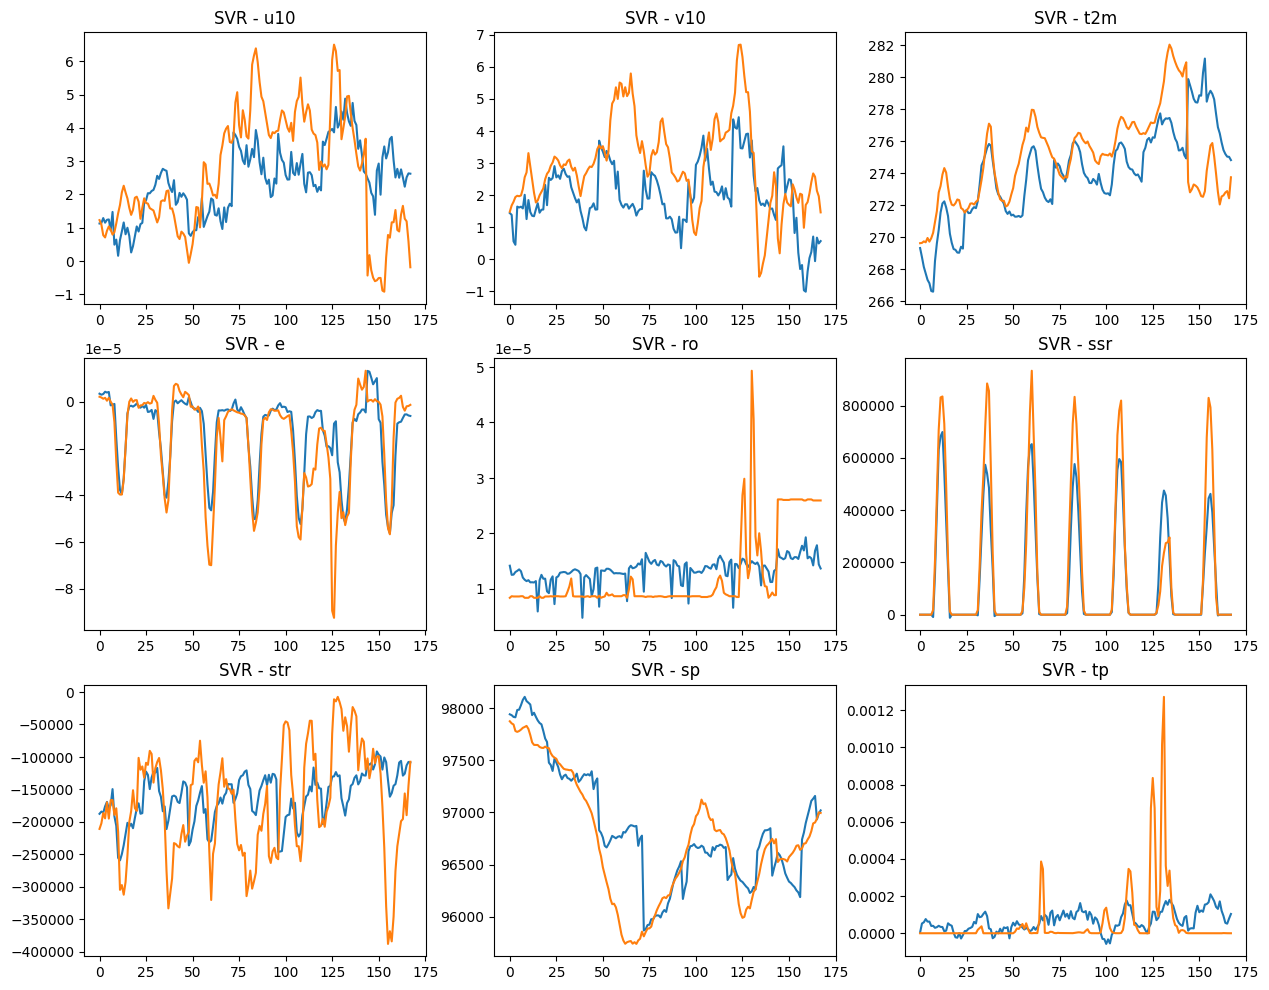
\includegraphics[width=\textwidth]{images/SVR_week.png}
    \caption{Przebiegi czasowe dla algorytmu SVR. Na żółto pokazane zostały dane 
    rzeczywiste, na niebiesko predykcje wygenerowane przez model}
    \label{svr-week}
\end{figure}

Dla perceptronu wielowarstwowego widać dużo większą wariancję w wyjściu modelu 
w zakresie krótkoterminowym. Duże wahania są szczególne widoczne dla wartości odpływów.
Bardzo możliwe, że charakterystyka oscylacyjna danych wejściowych  

\begin{figure}[H]
    \centering
    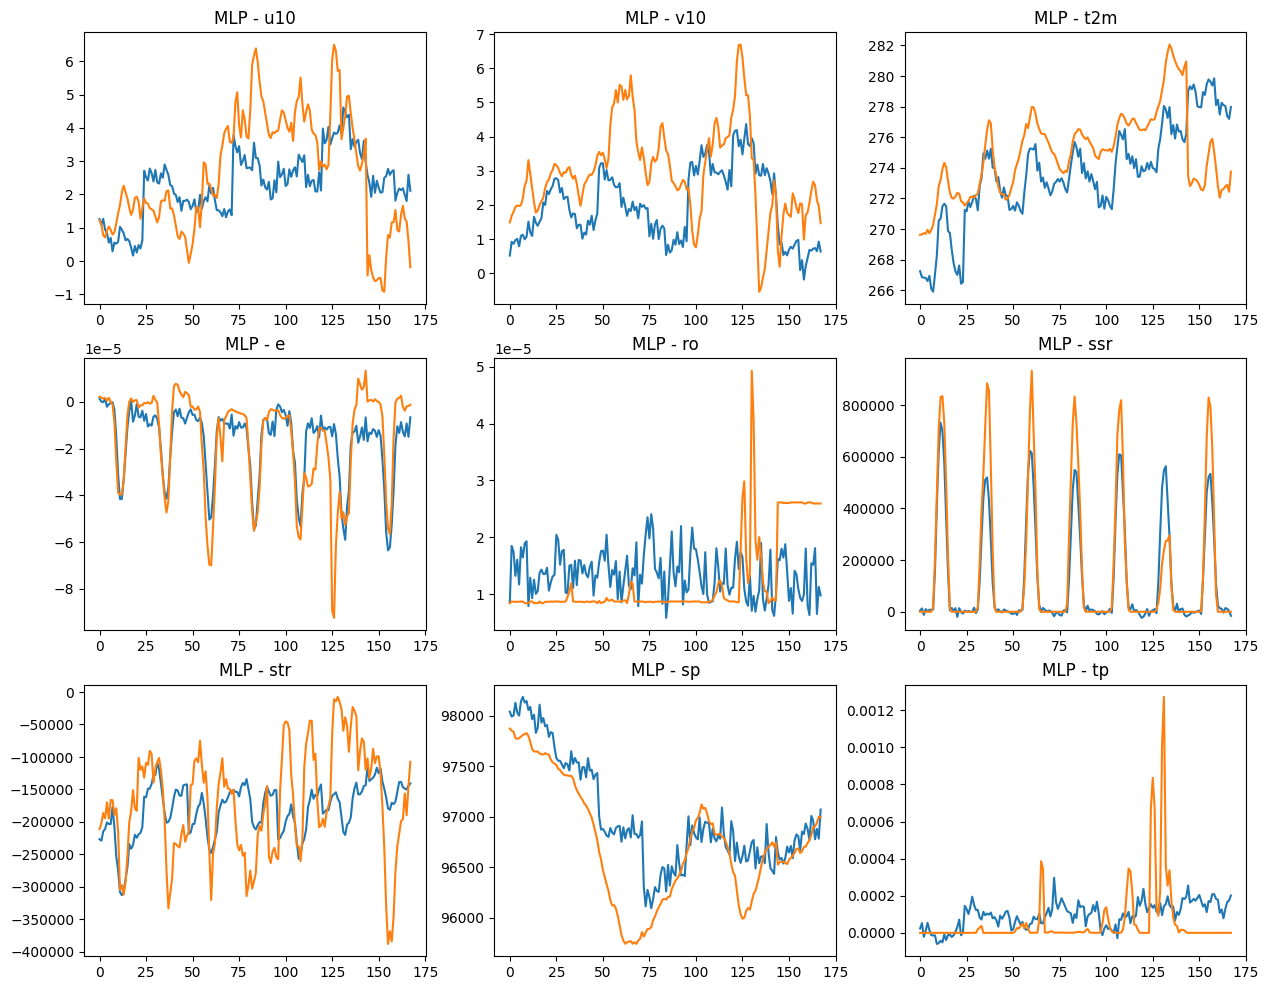
\includegraphics[width=\textwidth]{images/MLP_week.png}
    \caption{Przebiegi czasowe dla algorytmu MLP. Na żółto pokazane zostały dane 
    rzeczywiste, na niebiesko predykcje wygenerowane przez model}
    \label{mlp-week}
\end{figure}

\begin{figure}[H]
    \centering
    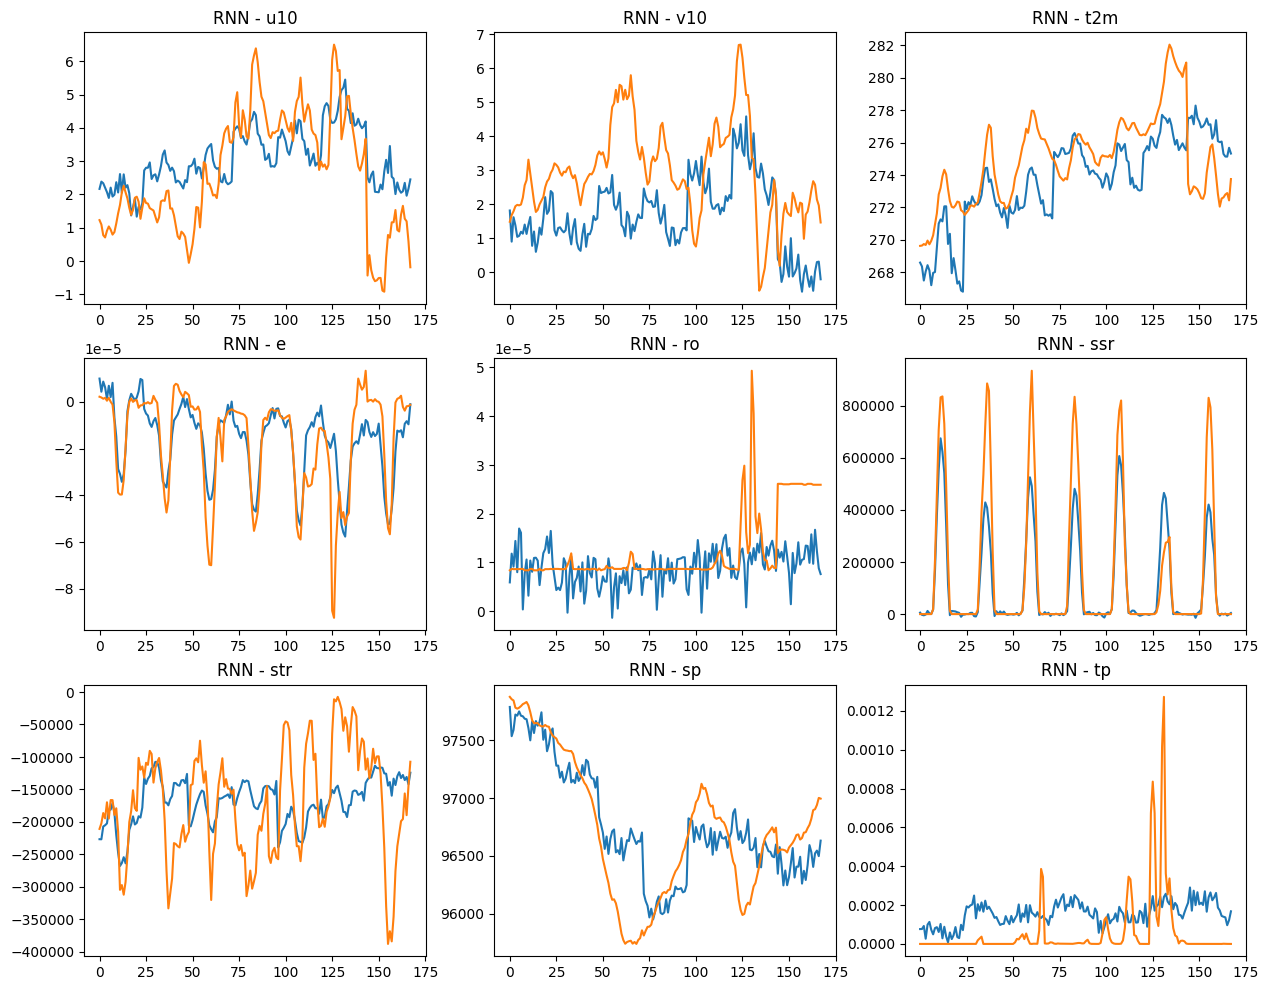
\includegraphics[width=\textwidth]{images/rnn_week.png}
    \caption{Przebiegi czasowe dla algorytmu RNN. Na żółto pokazane zostały dane 
    rzeczywiste, na niebiesko predykcje wygenerowane przez model}
    \label{rnn-week}
\end{figure}

\begin{figure}[H]
    \centering
    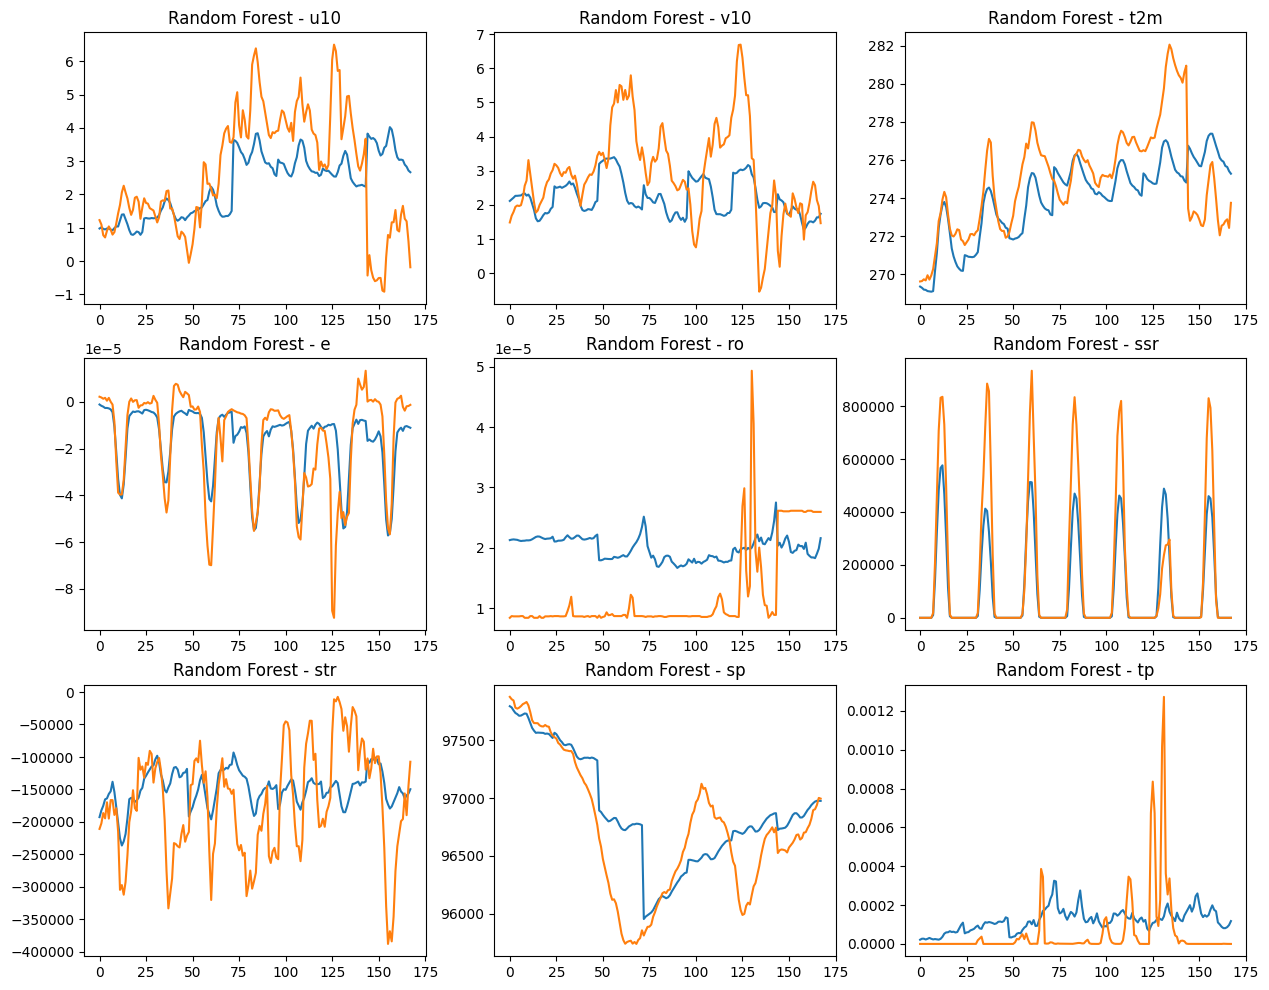
\includegraphics[width=\textwidth]{images/random_forest_week.png}
    \caption{Przebiegi czasowe dla algorytmu lasu losowego. Na żółto pokazane zostały dane 
    rzeczywiste, na niebiesko predykcje wygenerowane przez model}
    \label{forest-week}
\end{figure}

\begin{figure}[H]
    \centering
    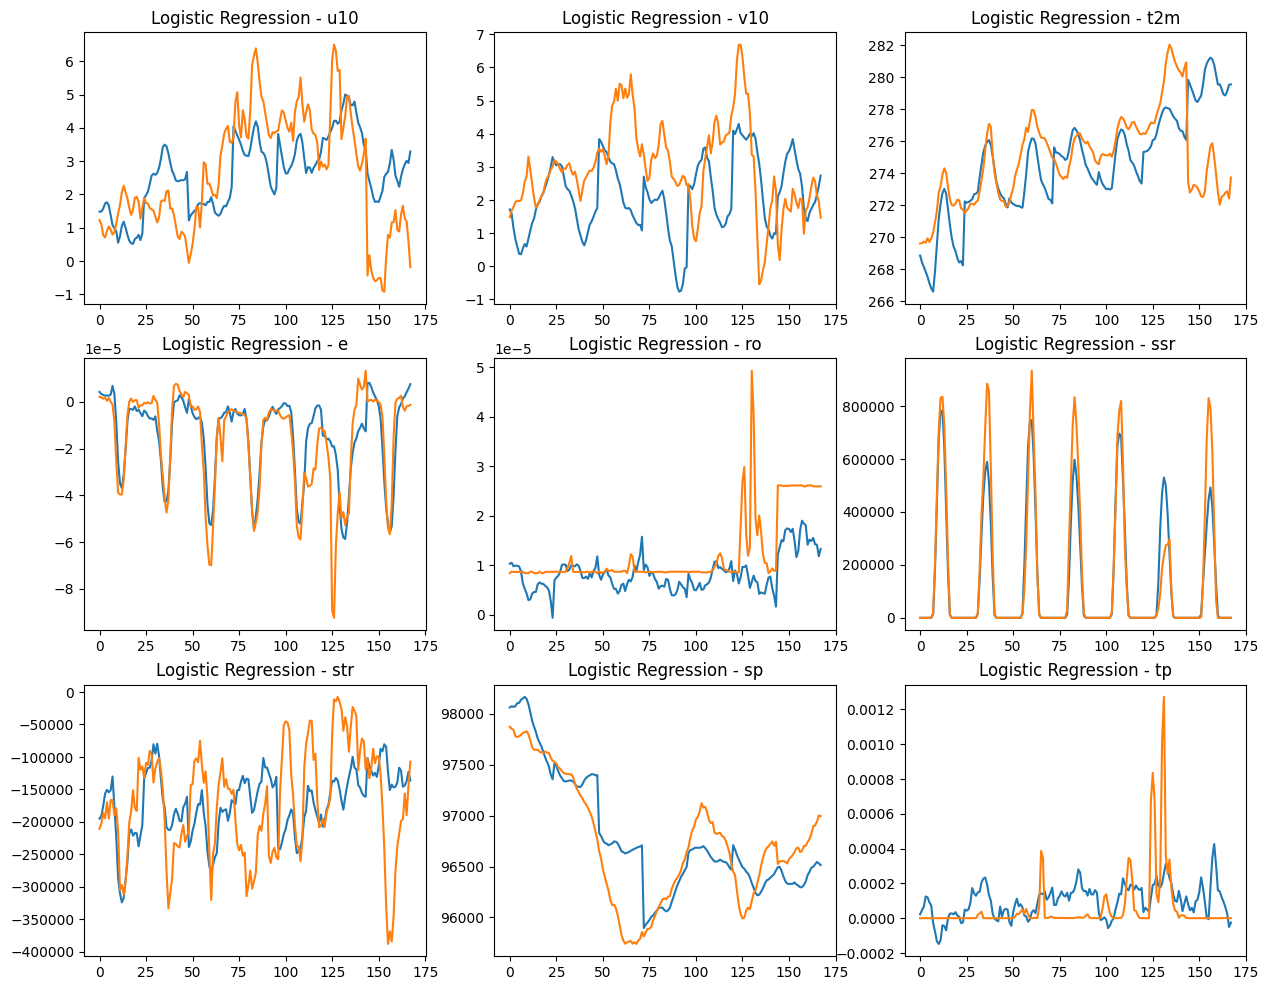
\includegraphics[width=\textwidth]{images/regression_week.png}
    \caption{Przebiegi czasowe dla algorytmu regresji logistycznej. Na żółto pokazane zostały dane 
    rzeczywiste, na niebiesko predykcje wygenerowane przez model}
    \label{regression-week}
\end{figure}

\begin{figure}[H]
    \centering
    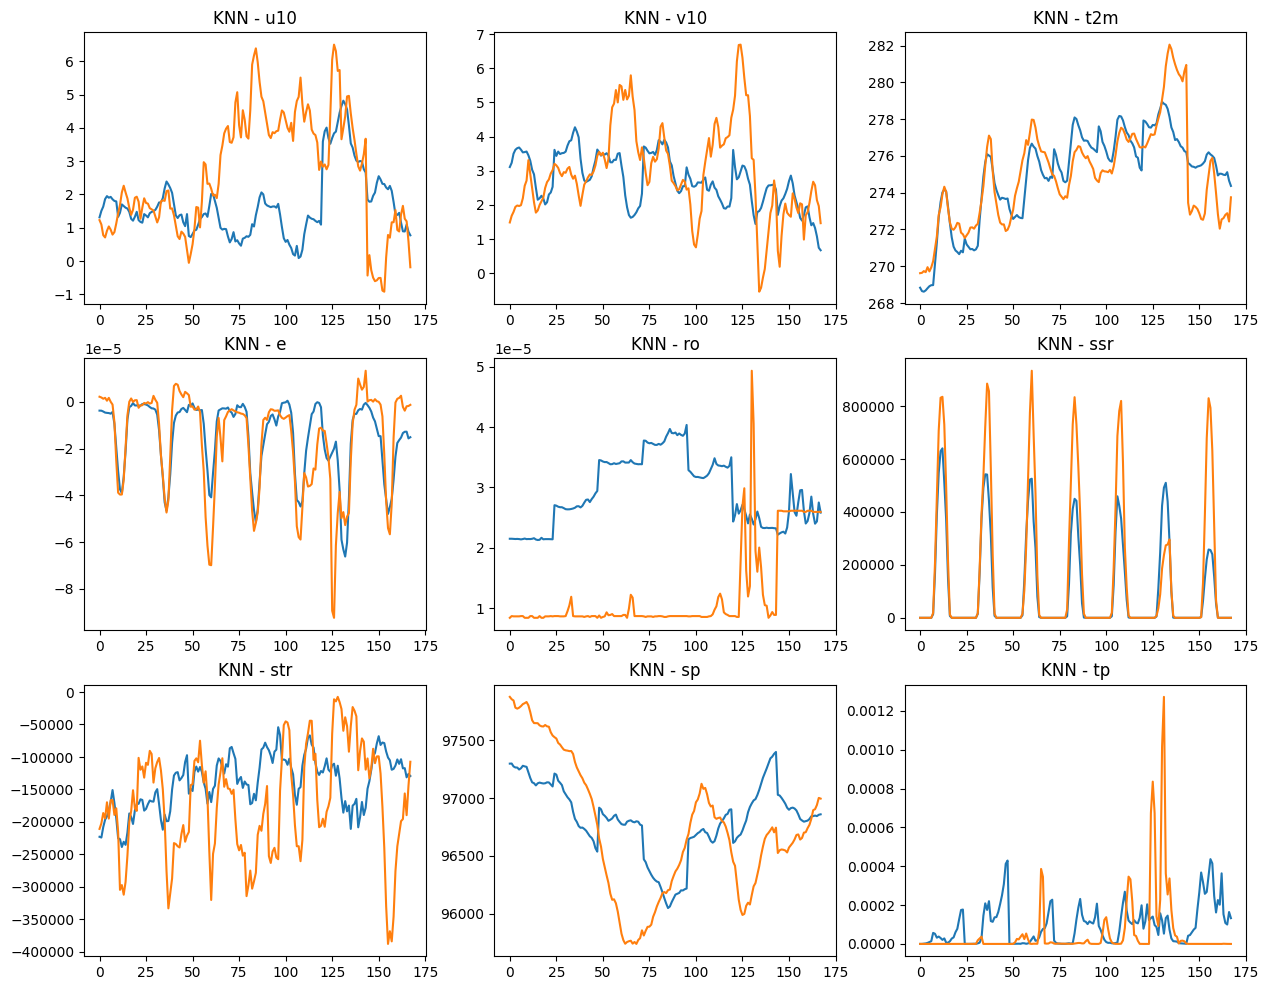
\includegraphics[width=\textwidth]{images/knn_week.png}
    \caption{Przebiegi czasowe dla algorytmu KNN. Na żółto pokazane zostały dane 
    rzeczywiste, na niebiesko predykcje wygenerowane przez model}
    \label{knn-week}
\end{figure}

\begin{figure}[H]
    \centering
    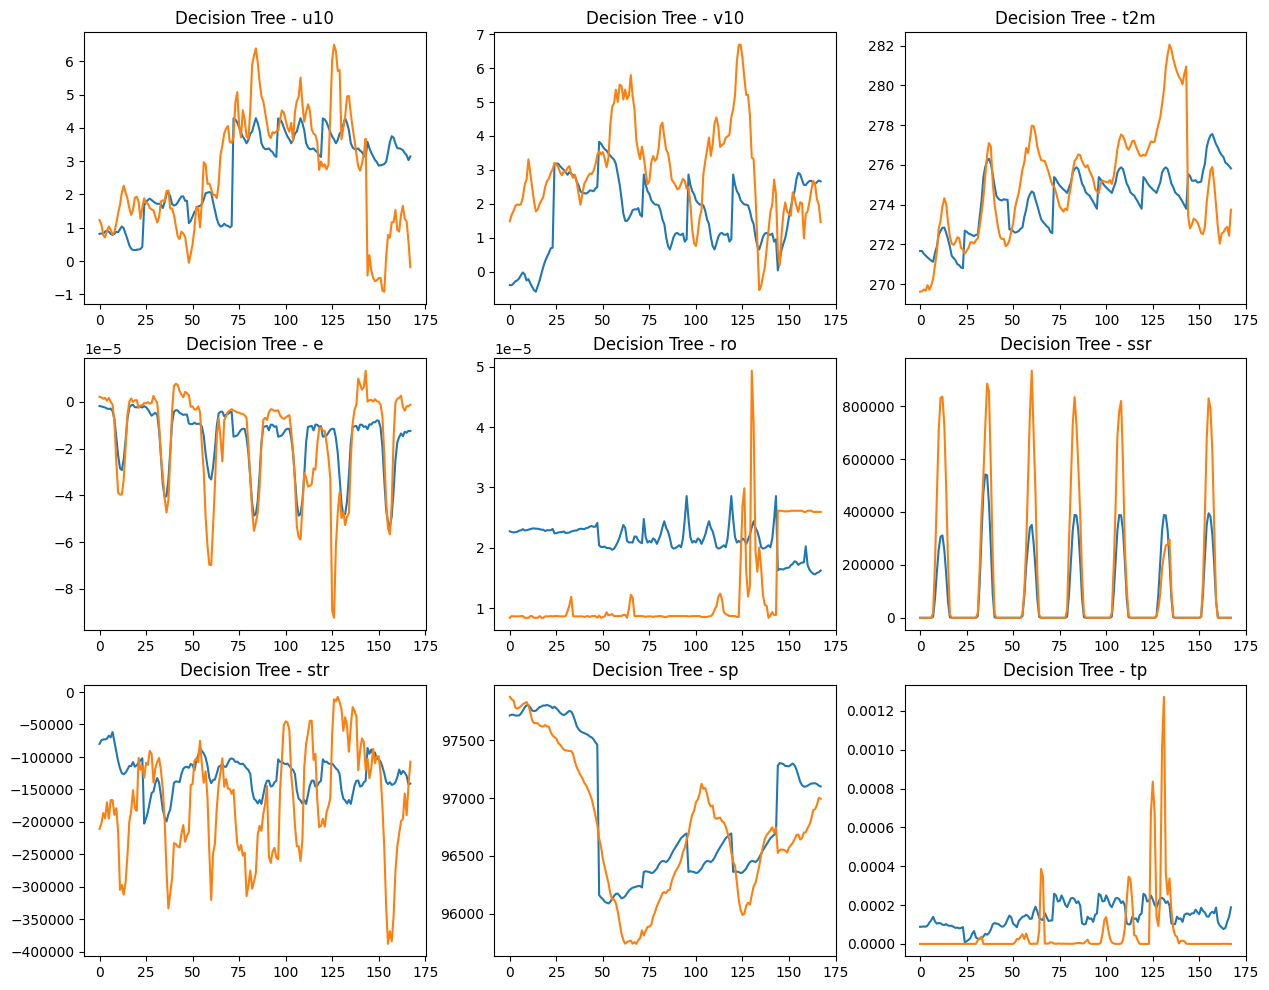
\includegraphics[width=\textwidth]{images/Decision_tree_week.png}
    \caption{Przebiegi czasowe dla algorytmu drzewa decyzyjnego. Na żółto pokazane zostały dane 
    rzeczywiste, na niebiesko predykcje wygenerowane przez model}
    \label{tree-week}
\end{figure}

\begin{figure}[H]
    \centering
    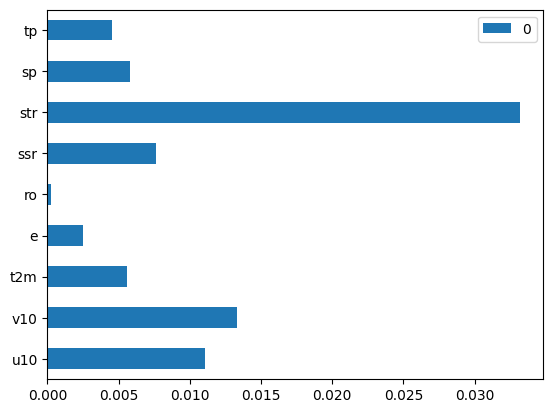
\includegraphics[width=\textwidth]{images/svr_mse_bar.png}
    \caption{}
    \label{svr-mse-bar}
\end{figure}

\begin{figure}[H]
    \centering
    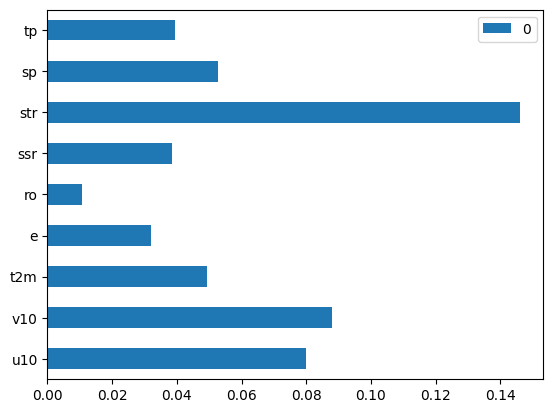
\includegraphics[width=\textwidth]{images/svr_mae_bar.png}
    \caption{}
    \label{svr-mae-bar}
\end{figure}

% Inferential statistics: Report the results of any inferential 
% statistical analyses that you conducted to test your research 
% hypotheses, such as t-tests, ANOVA, regression analysis, or 
% other statistical tests. Be sure to include the statistical 
% significance of the results and the effect sizes.
\subsection{Testy statystyczne}

\begin{figure}[H]
    \centering
    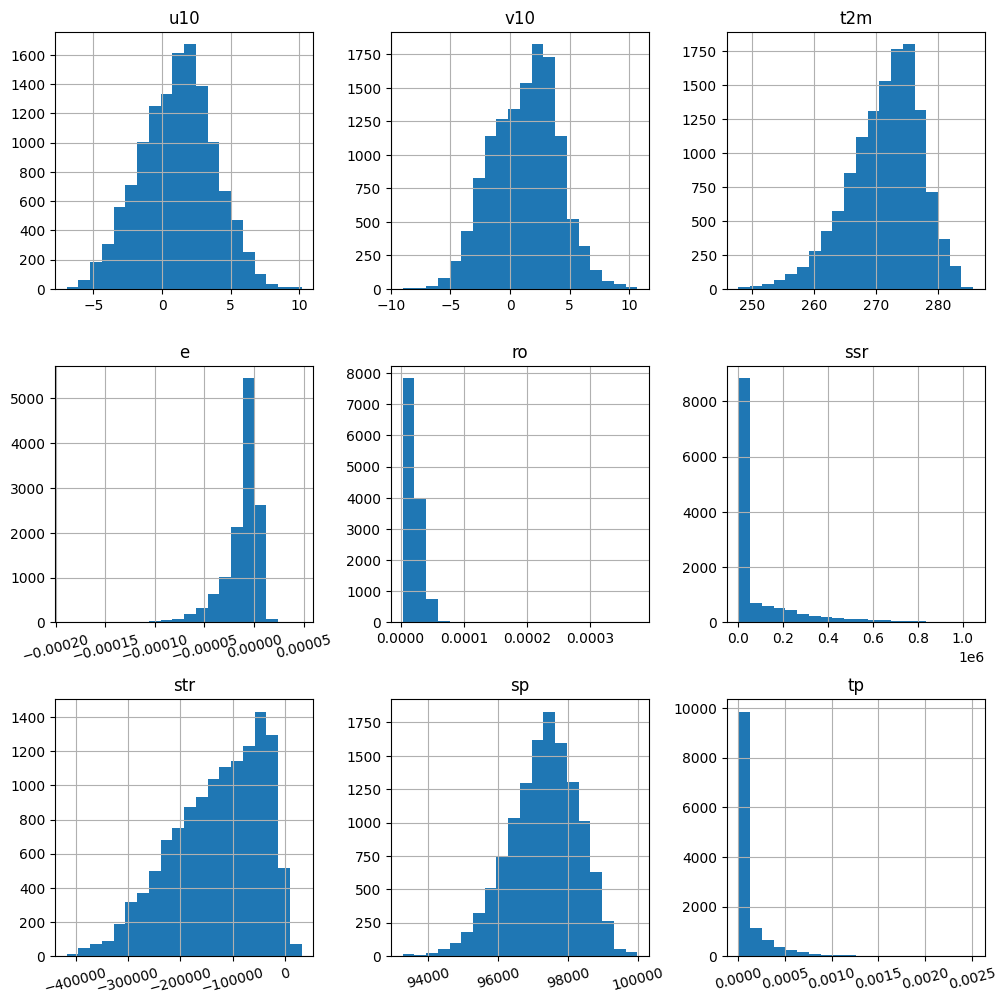
\includegraphics[width=\textwidth]{images/hist.png}
    \caption{}
    \label{real-hist}
\end{figure}

\begin{figure}[H]
    \centering
    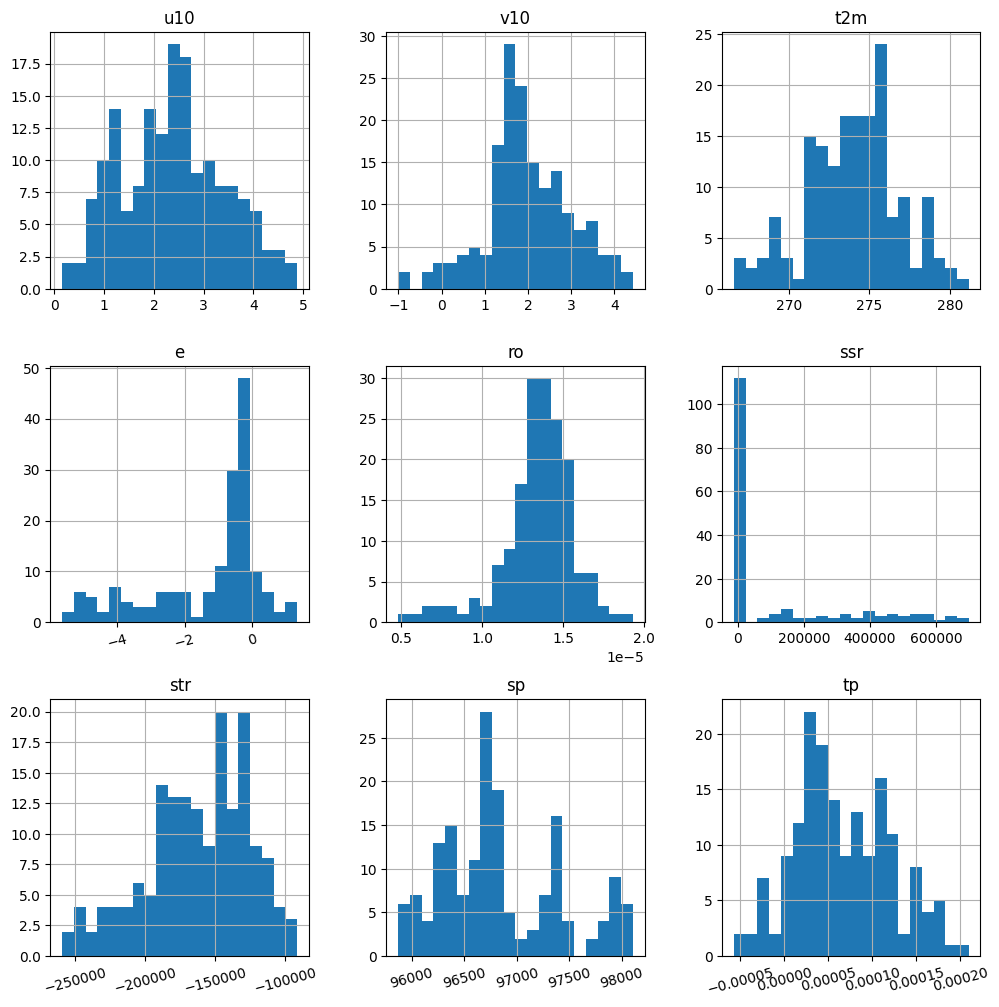
\includegraphics[width=\textwidth]{images/svr_hist.png}
    \caption{}
    \label{svr-hist}
\end{figure}

\begin{figure}[H]
    \centering
    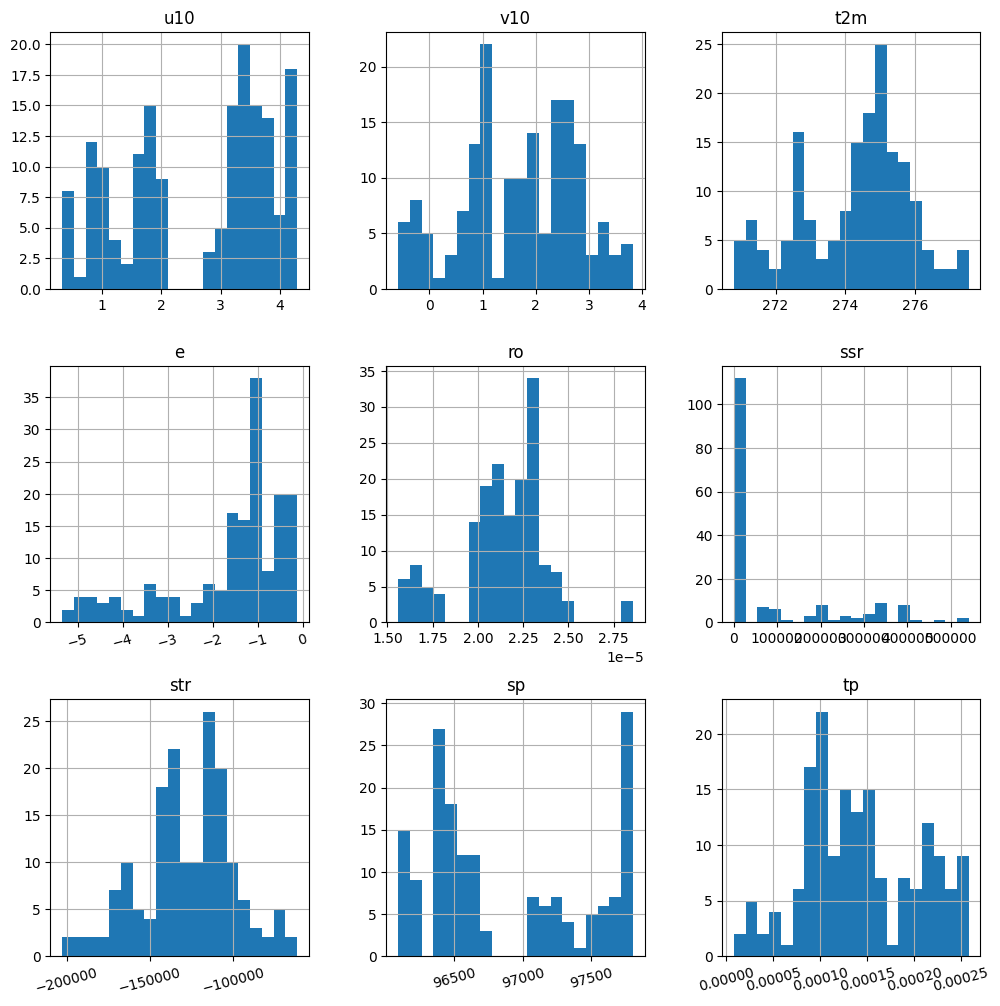
\includegraphics[width=\textwidth]{images/dt_hist.png}
    \caption{}
    \label{dt-hist}
\end{figure}

\begin{figure}[H]
    \centering
    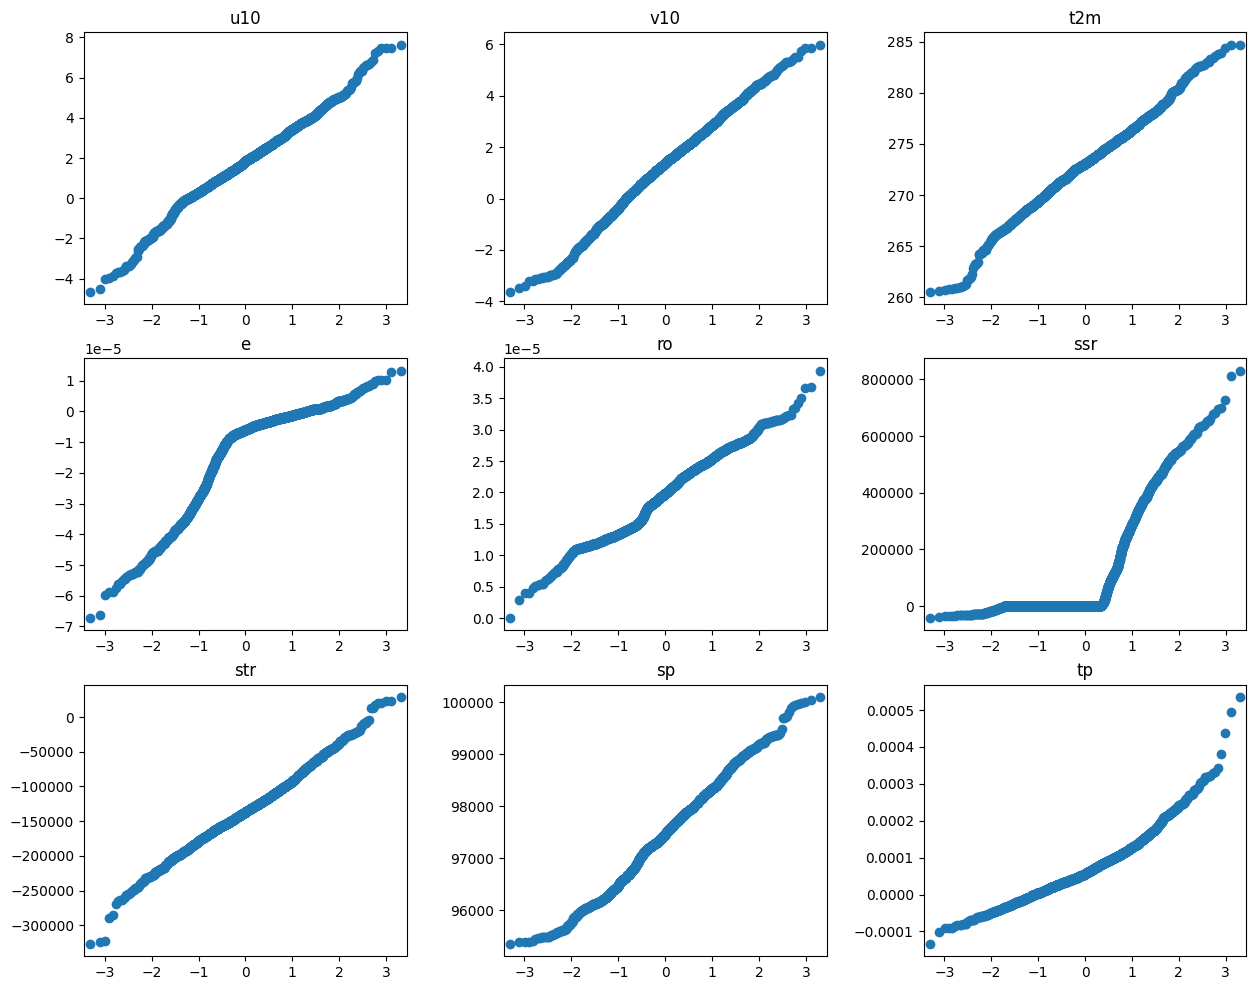
\includegraphics[width=\textwidth]{images/svr_qq.png}
    \caption{}
    \label{svr-qq}
\end{figure}

\begin{figure}[H]
    \centering
    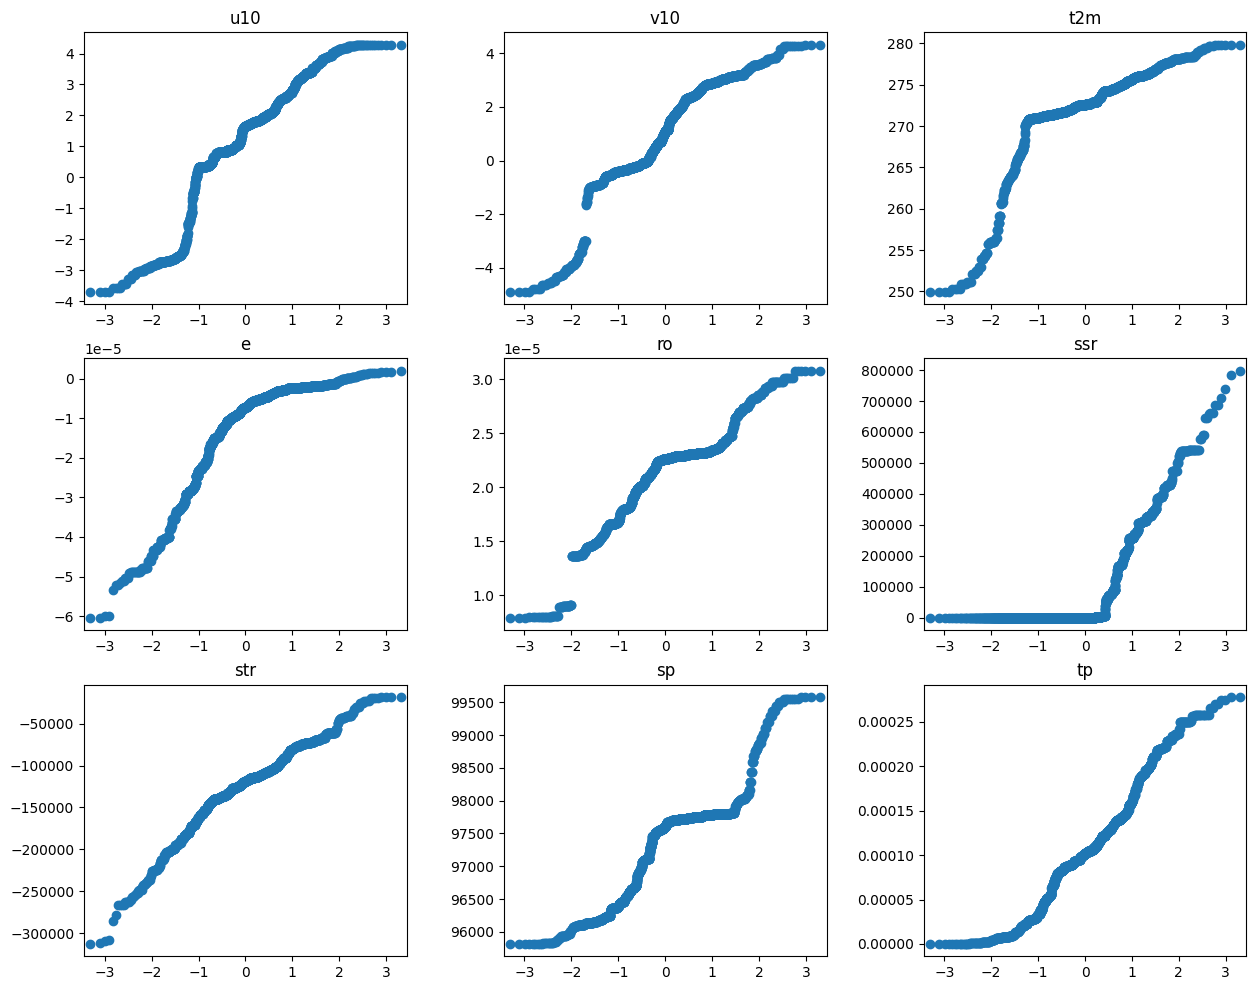
\includegraphics[width=\textwidth]{images/dt_qq.png}
    \caption{}
    \label{dt-qq}
\end{figure}

\begin{figure}[H]
    \centering
    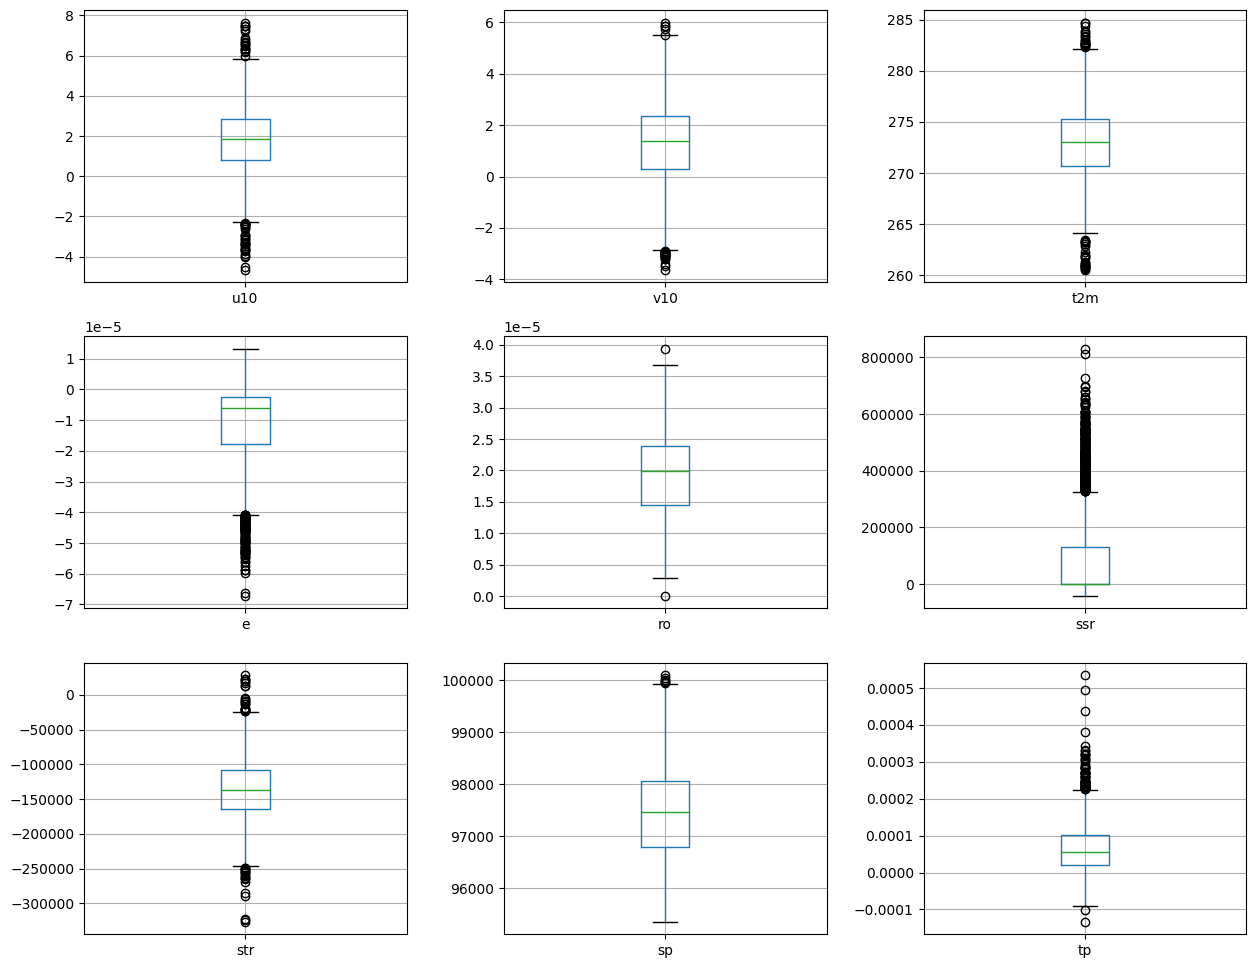
\includegraphics[width=\textwidth]{images/svr_box.png}
    \caption{}
    \label{svr-box}
\end{figure}

\begin{figure}[H]
    \centering
    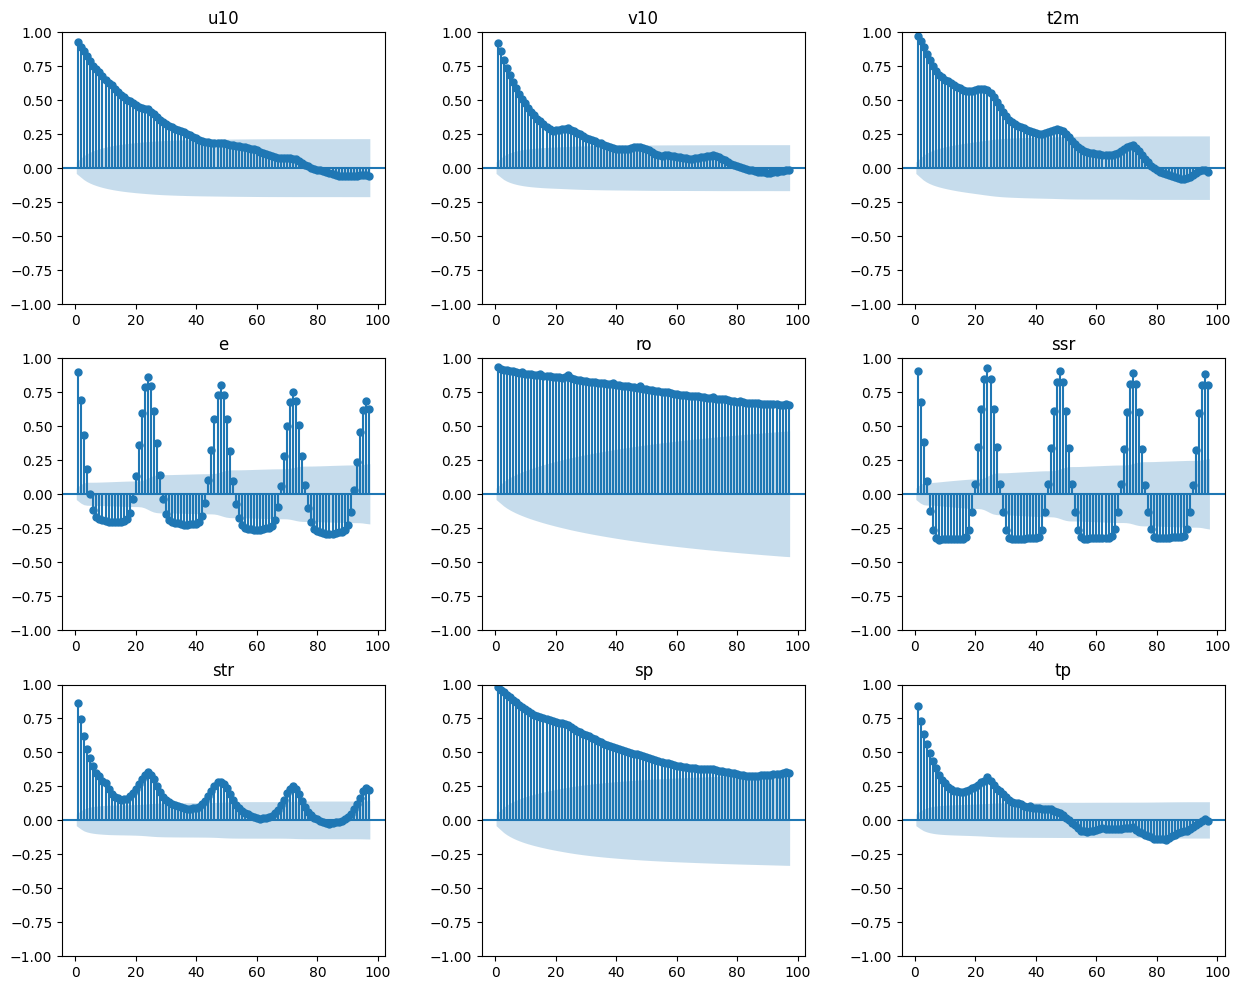
\includegraphics[width=\textwidth]{images/svr_autocorr.png}
    \caption{}
    \label{svr-autocorr}
\end{figure}

\begin{figure}[H]
    \centering
    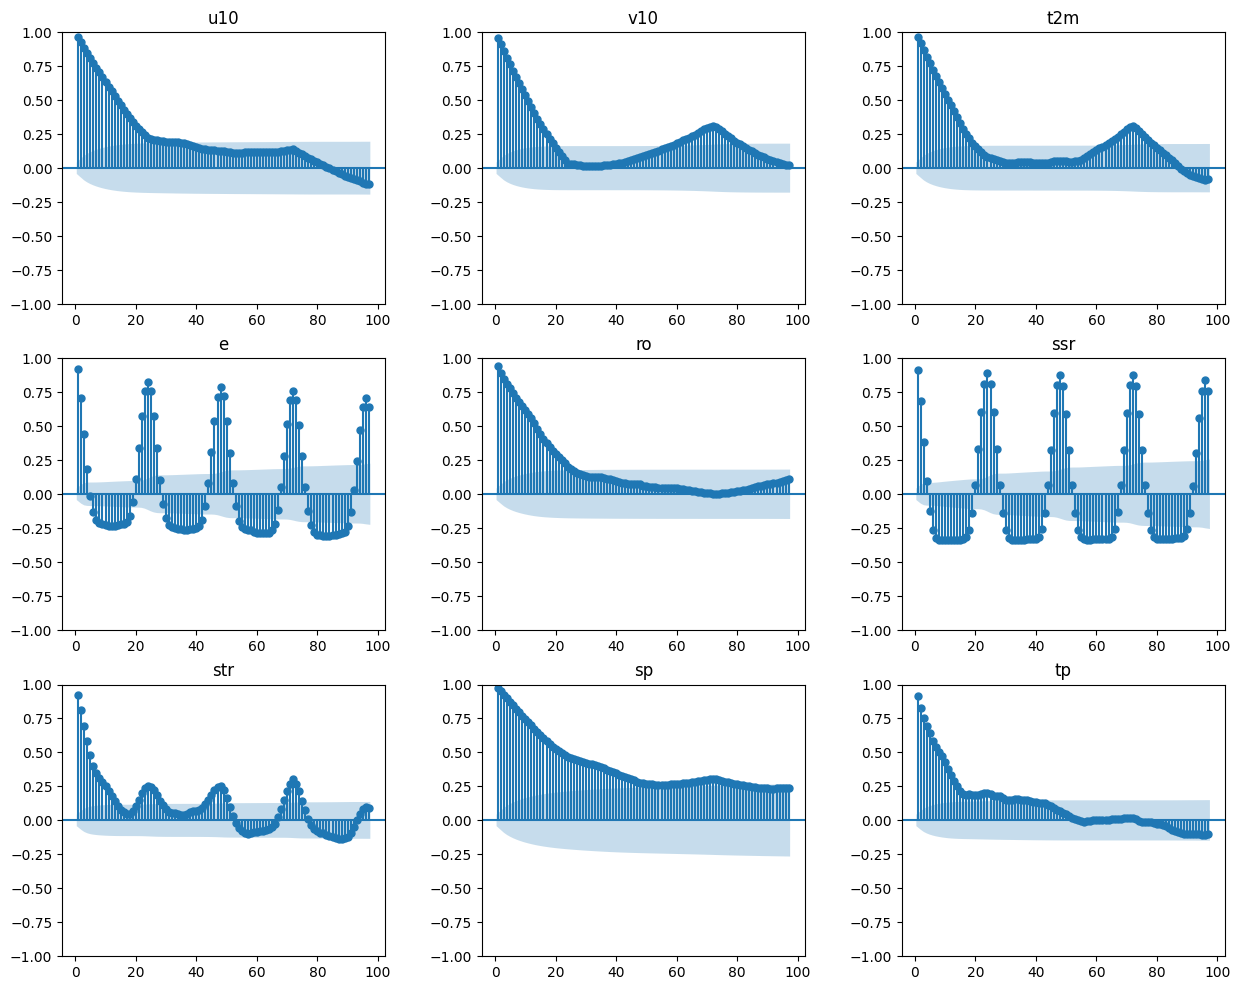
\includegraphics[width=\textwidth]{images/dt_autocorr.png}
    \caption{}
    \label{dt-autocorr}
\end{figure}

\begin{figure}[H]
    \centering
    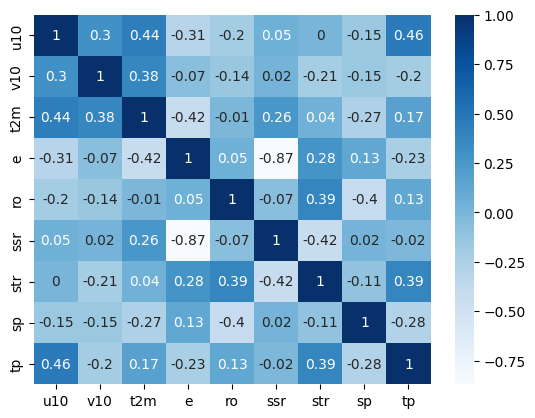
\includegraphics[width=\textwidth]{images/svr_corr_matrix.png}
    \caption{}
    \label{svr-corr-matrix}
\end{figure}

\begin{figure}[H]
    \centering
    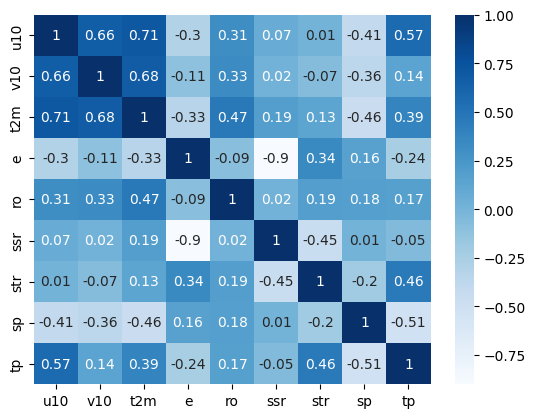
\includegraphics[width=\textwidth]{images/dt_corr_matrix.png}
    \caption{}
    \label{dt-corr-matrix}
\end{figure}


% Tables and figures: Present your data in tables and figures 
% that are clear, concise, and easy to read. Ensure that your 
% tables and figures are properly labeled and that they effectively 
% illustrate your findings.

% Subgroup analyses: Conduct subgroup analyses if relevant to 
% your research questions. For example, if you are comparing the 
% performance of different machine learning models, you might conduct 
% subgroup analyses based on the type of model used or the size of the training data.
\subsection{Porównanie modeli}

\begin{figure}[H]
    \centering
    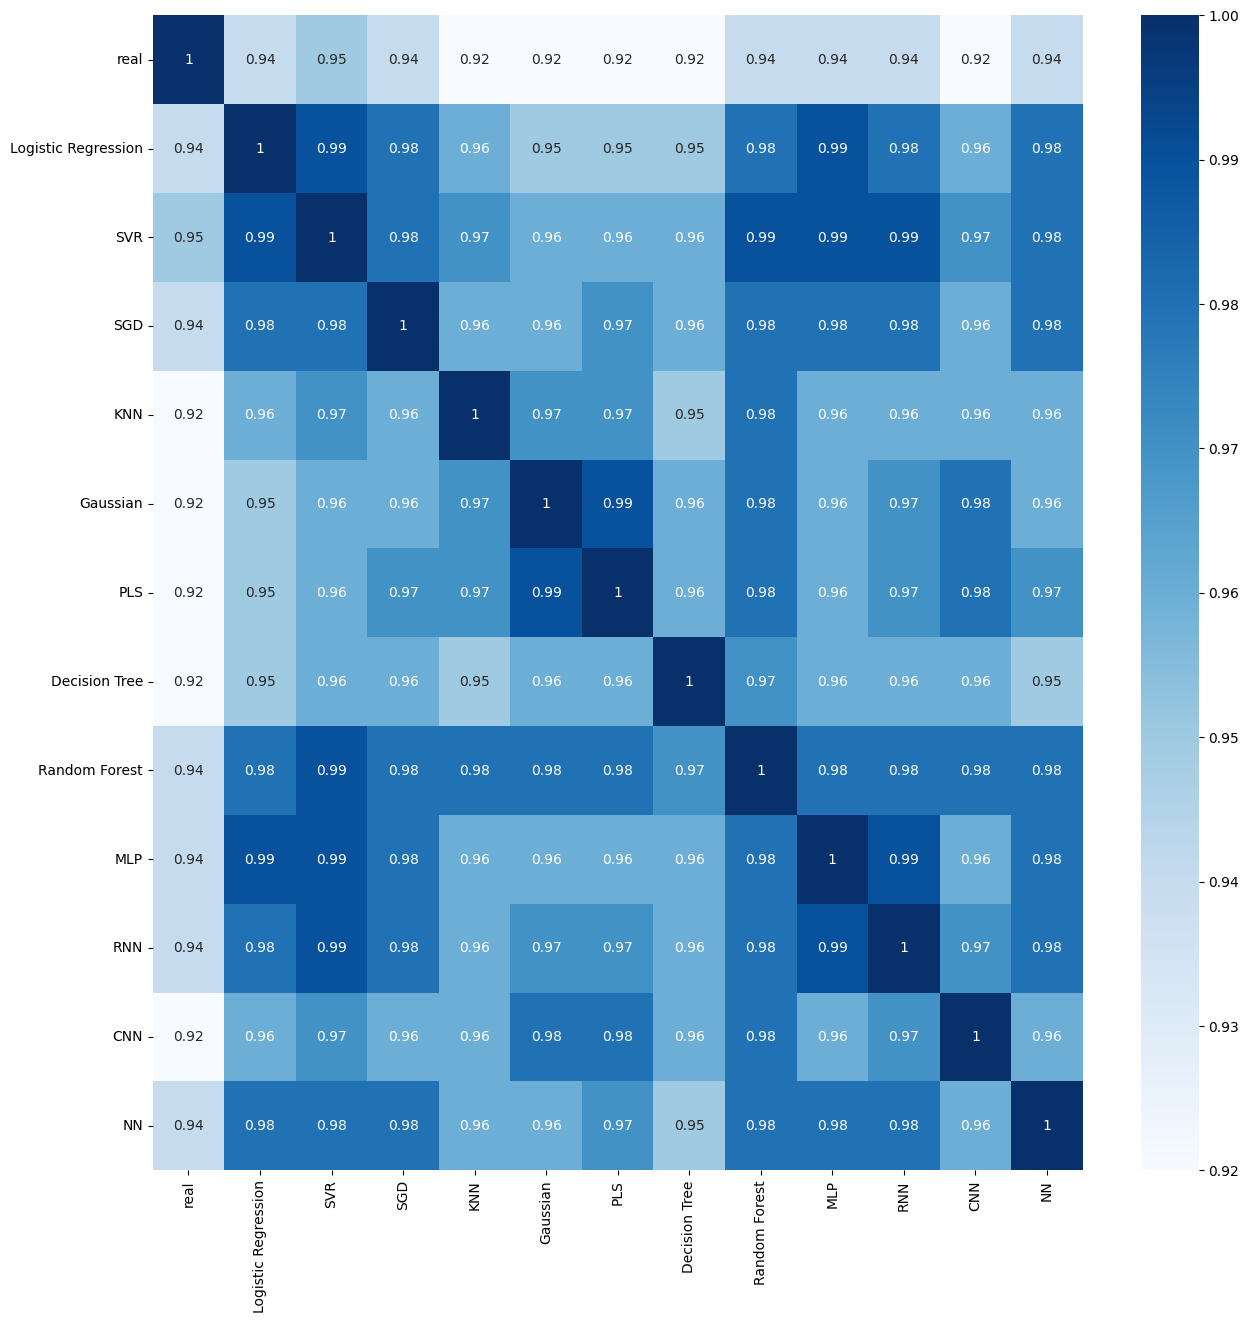
\includegraphics[width=\textwidth]{images/pred_corr.png}
    \caption{}
    \label{pred_corr}
\end{figure}

\begin{figure}[H]
    \centering
    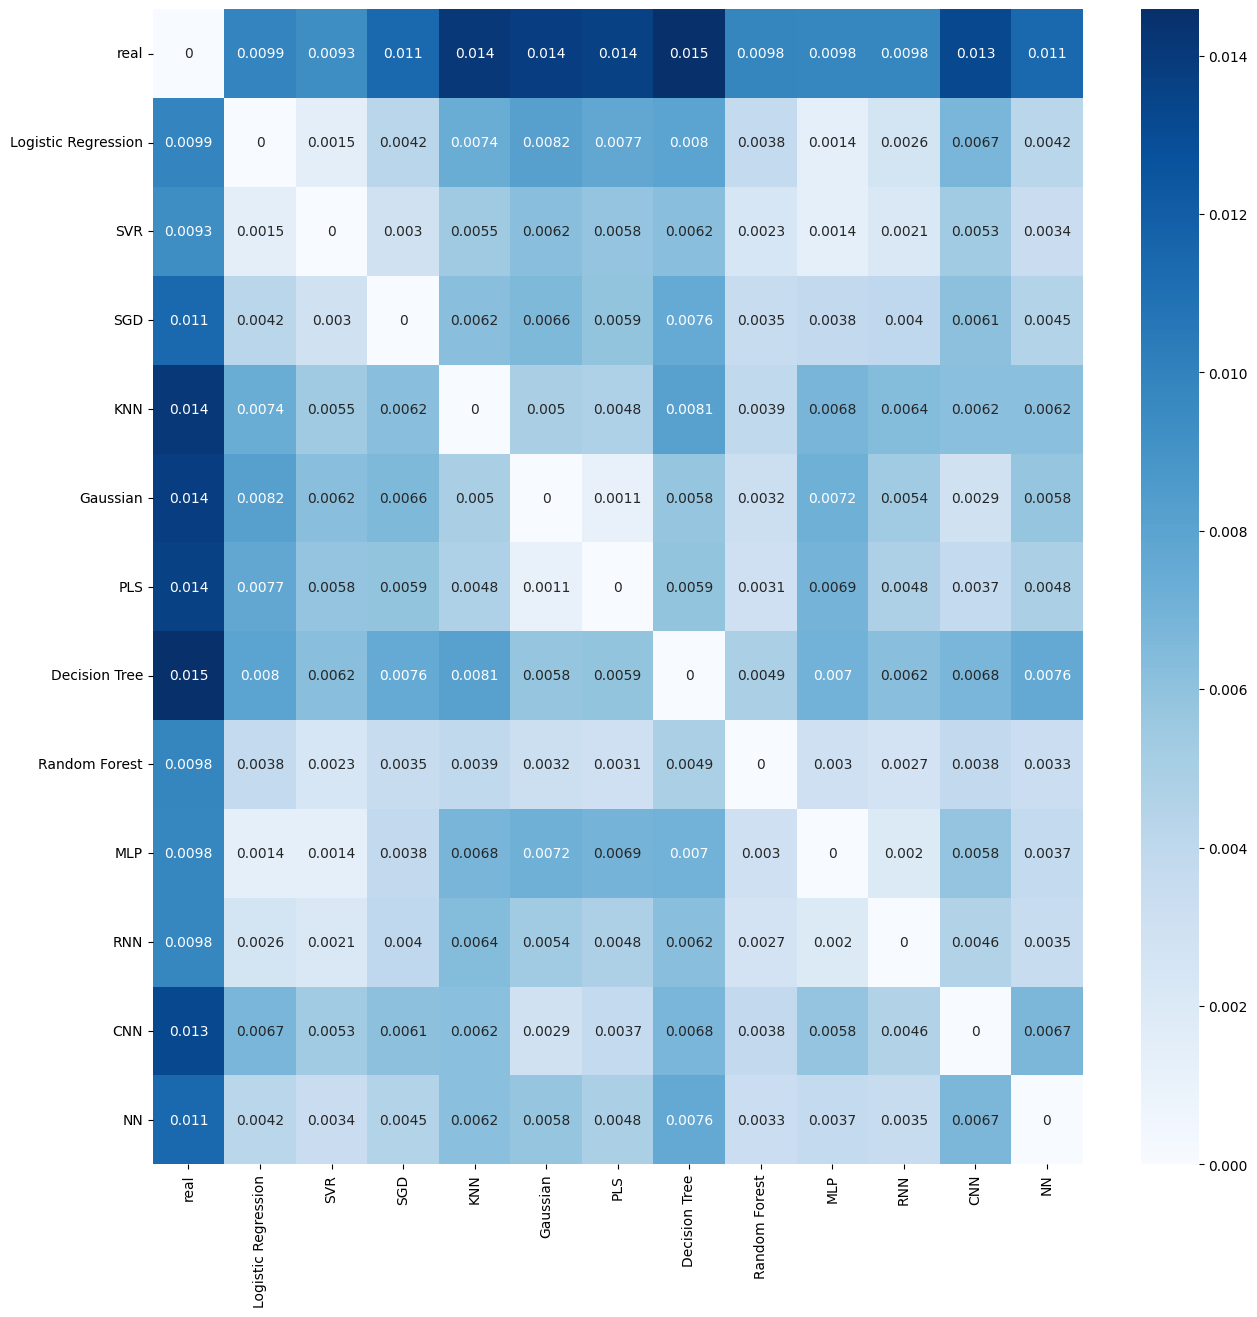
\includegraphics[width=\textwidth]{images/mse_matrix.png}
    \caption{}
    \label{mse-matrix}
\end{figure}

\begin{figure}[H]
    \centering
    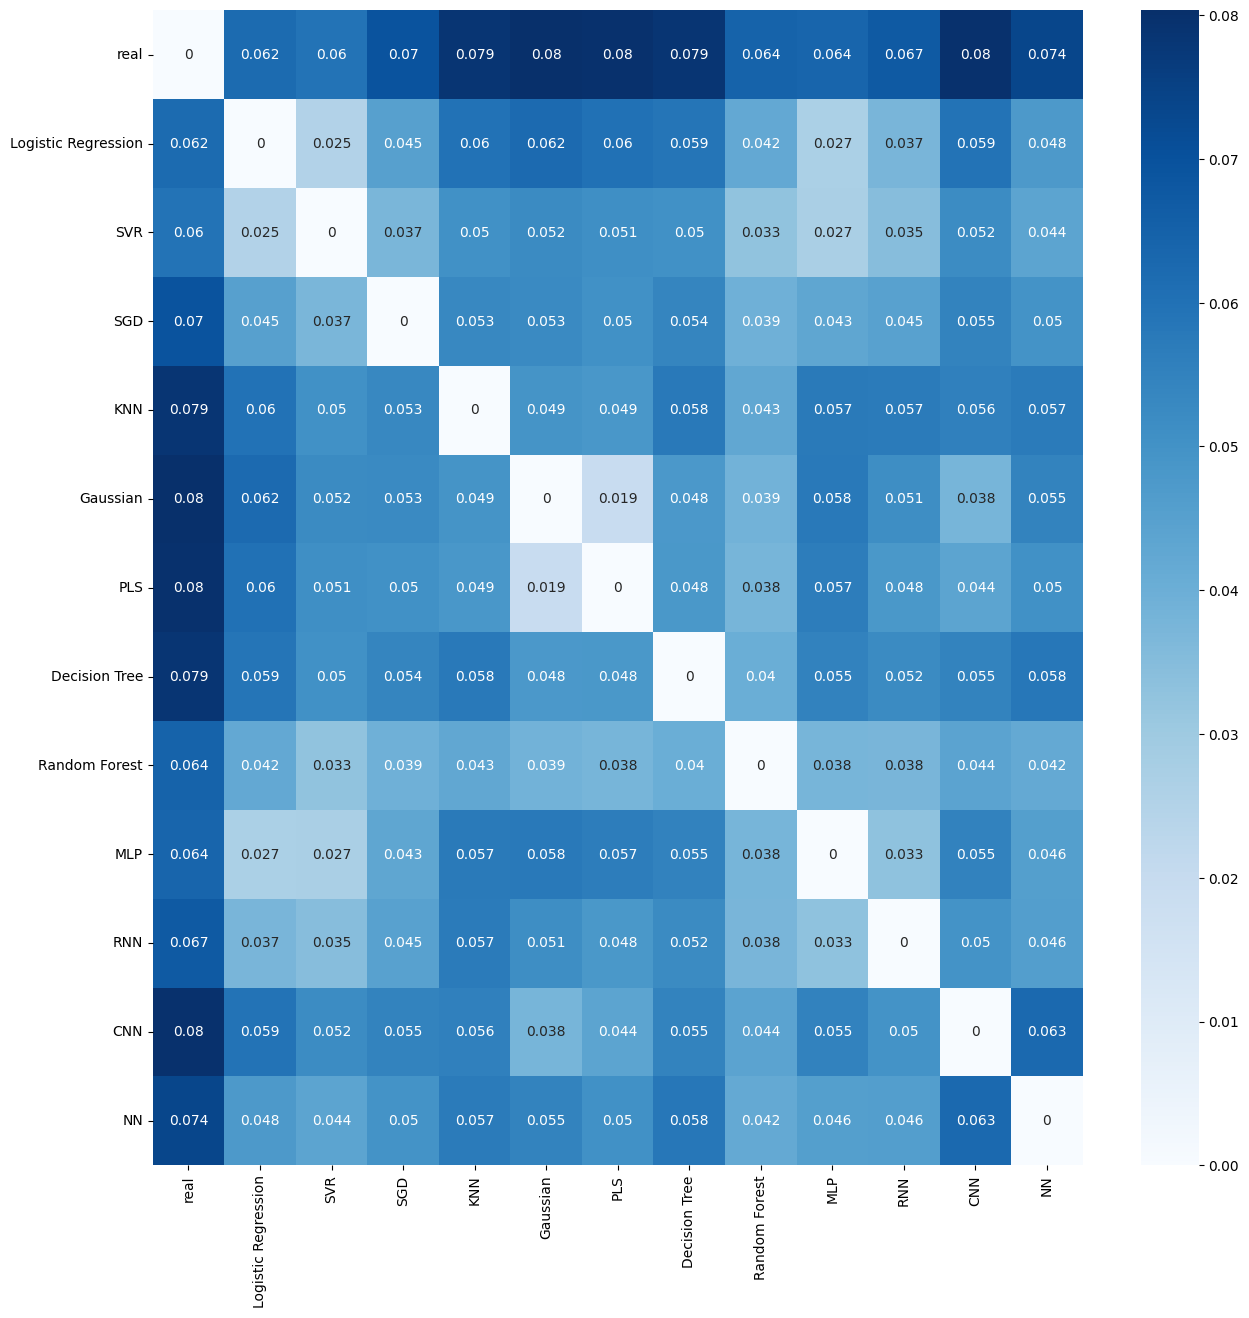
\includegraphics[width=\textwidth]{images/mae_matrix.png}
    \caption{}
    \label{mae-matrix}
\end{figure}


\begin{figure}[H]
    \centering
    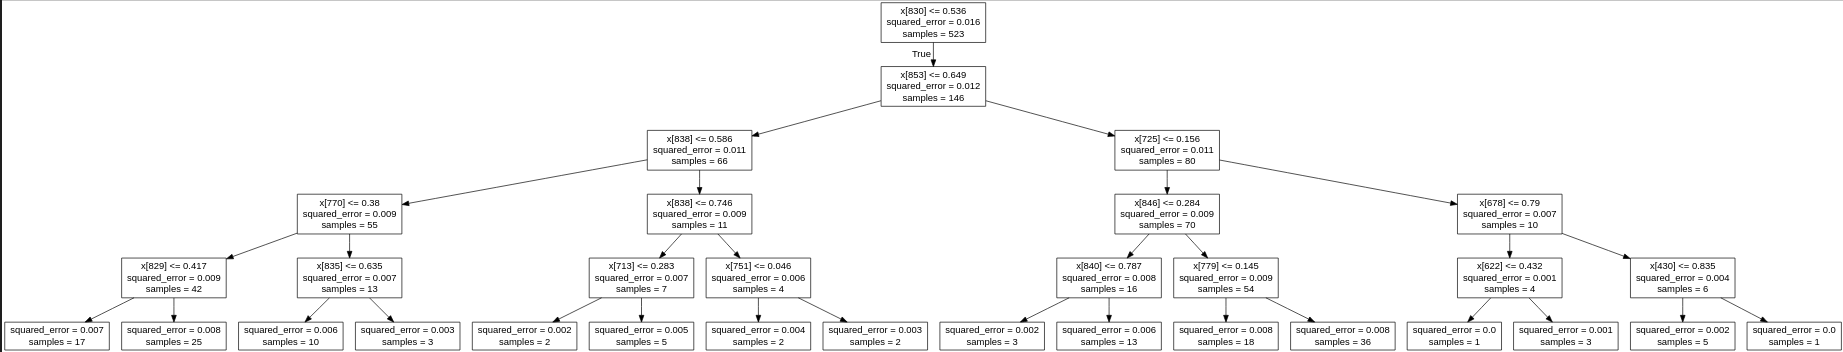
\includegraphics[width=\textwidth]{images/tree.png}
    \caption{}
    \label{tree-graph}
\end{figure}

% Interpretation: Provide an interpretation of your findings and 
% relate them back to your research questions or hypotheses. Discuss 
% the implications of your results for the broader field of weather 
% prediction and the use of artificial intelligence and machine learning 
% techniques in this area.
\subsection{Interpretacja}

% Limitations: Discuss any limitations of your study that may 
% have affected the validity or generalizability of your findings. 
% Be sure to acknowledge any potential sources of bias or confounding variables.
\subsection{Ograniczenia}